\section{Disorder and Random Systems}

\subsection{Introduction and Motivation}
Disorders and imperfections are unavoidable in real systems; do phase transitions still exist in this setting? This will be the first point which we will address, and we will be able to answer it quite sharply.

The answer will turn out to be yes, but we then have the follow-up question; how are the transitions modified? We will find that the (upper and lower) critical dimensions become modified.

Finally, we may ask if there will be new phenomena emerging from disorder; indeed there can be, and we will look at the example of a glass, where there is an abrupt transition to being frozen/carrying information.


\subsection{Disorder Type I - Impurities/Vacancies}
E.g. we have a ferromagnet, and randomly start removing spins. We could for example write down the Hamiltonian:
\begin{equation}
    H(\set{s},\set{m}) = -\frac{1}{2}\sum_{ij}J_{ij}s_is_jm_im_j
\end{equation}
where randomly, we pick sites $m_i$ and set them to zero such that those terms become absent from the sum. We will need to make a careful distinction about whether the system is quenched or annealed. Suppose we ``freeze in'' the spin configuration. Then the partition function looks like:
\begin{equation}
    Z(\set{m}) = \Tr_S e^{-\beta H(s, m)}
\end{equation}
which is called ``quenched''. This has the odd feature that the answer depends explicitly on the $\set{m}$. If we do the experiment again and put the impurities in different places, we get a different partition function. We could instead construct the ``annealed'' partition function, which is:
\begin{equation}
    Z = \Tr_m Z(\set{m})
\end{equation}
where we average over all configurations $\set{m}$ of empty sites. The annealed problem is a tough one and we won't address it in this lecture, but we will attack the quenched partition function.

A comment - we lose translational invariance when we do this.

Let us block our system. We can consider an averaged free energy:
\begin{equation}
    \bar{F} = \Tr_m Z[\set{m}]F[\set{m}]
\end{equation}
where we assume that we can compute (over a given block) $F[\set{m}]$ governed by $P[\set{m}]$ (each block will have a different value, but obeys the same distribution). The $\bar{F}$ above represents a quenched average. Looking at the probability distribution, we have:
\begin{equation}
    P[\set{m}] = \prod_i \left[(1 - x)\delta_{m_i 1} + x \delta_{m_i0}\right]
\end{equation}
where $x$ is is the concentration of vacancies. The important thing to think about; when we do the trace over $S$, we average over spin configurations, but do not minimize over the free energy. It is instead, fixed here.

We distinguish the thermal average with the spatial average:
\begin{equation}
    \avg{s_is_j} \neq \overline{\avg{s_is_j}}
\end{equation}
where the lhs represents the thermal average, the rhs the spatial. The thermal average is dependent on the spin configuration, but the spatial average only depends on the distance between $i, j$ i.e. $\abs{i - j}$. Formally, we can write:
\begin{equation}
    \overline{\avg{s_is_j}} = \frac{1}{N}\sum_k \avg{s_{k+i}, s_{k+j}} = M(\abs{i-j})
\end{equation}
why might we want to do this? It is relevant for determining magnetic fluctuations in the system.

We can consider some types of impurities/vacancies:
\begin{enumerate}[(i)]
    \item Bond dilution, e.g. $J_{ij} = J + \text{small fluctuations}$.
    \item Random field; $H = \sum_{ij}J_{ij}s_is_j + \sum_i h_i s_i$ where we make the $h_i$ random. Where $\bar{h} = 0$ and $\overline{hh} = \Delta$.
    \item Spin glass, where we take $J_{ij}$ random with mean zero. In this case, since we pick couplings randomly, we can have frustrated systems. Note that is similar to bond dilution with $J = 0$, but allowing the fluctuations to be not necessarily small. We could call a system with $s_i(0)s_i(t) \neq 0$ a glass (correlations get ``baked in'').
\end{enumerate}

\subsection{Computing quenched averages - Replica Trick}
We want to compute:
\begin{equation}
    \bar{F} = \Tr_m P[\set{m}]\ln Z[\set{m}]
\end{equation}
averaging logarithms is hard, but we can expand $\ln Z$ in a power series:
\begin{equation}
    \ln Z = \lim_{n \to 0}\frac{Z^n - 1}{n}
\end{equation}
Taking quenched averages of power series of $Z$ are much easier. We interpret this as taking our Hamitonian and \emph{replicating}it:
\begin{equation}
    \overline{Z^n} = \Tr_m \Tr_{s^a} P[\set{m}] e^{-\sum_{a=1}^n H[\set{s^a}, \set{m}]}
\end{equation}
Because $P[\set{m}]$ is random, this will correspond to some SM model with randomness. But the trick is that we can now do the average over $m$ first, so we end up with:
\begin{equation}
    \overline{Z^n} = \Tr_{s^a}e^{-\sum_{ab}H_{\text{eff}(s^a, s^b)}}
\end{equation}
where by doing the average over $m$ we get correlations between the different replicas. (Note that in principle we could have couplings between higher numbers of replicas, but since we started with two-body couplings, we have at most couplings between pairs of replicas).

\subsection{Transition Temperatures and Concentration}
Suppose I have some concentration of impurities $x \ll 1$, and the transition temperature $T_c$ depends on $x$. Therefore, we have:
\begin{equation}
    T_c(x) \implies \xi \sim \abs{T - T_c(x)}^{-\nu(x)}
\end{equation}
Because the system varies spatially, the concentration may be different at different locations. We thus may consider the deviation:
\begin{equation}
    \delta T_c(\v{r}) = T_c(\v{r}) - T_c
\end{equation}
Let us define a correlation function:
\begin{equation}
    W(\v{r} - \v{r}') = \overline{T_c(\v{r})T_c(\v{r}')}
\end{equation}
We now ask; as we open up the block size of the system, what happens to the correlation function?

We consider an aperture/block size $L$ such that $a \ll L \ll \text{system size}$. Then:
\begin{equation}
    (\Delta T_c)^2 = \int_a^L \frac{d^dr}{L^d}\int_a^{r_0}\frac{d^dr'}{L^d}W(\v{r} - \v{r}')
\end{equation}
where we integrate up to a characteristic length scale of the correlation $r_0$:

\begin{center}
    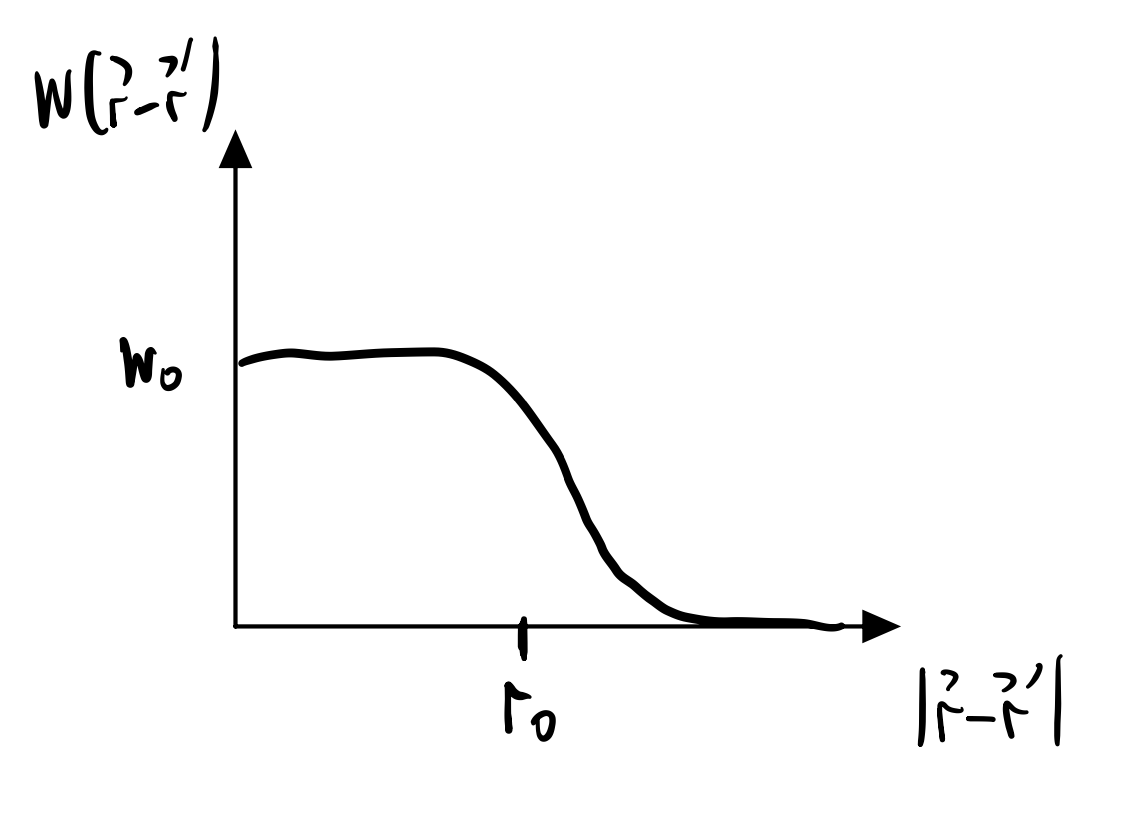
\includegraphics[scale=0.4]{Lectures/Figures/lec12-corr.png}
\end{center}

We then find;
\begin{equation}
    \Delta T_c \sim W_0^{1/2}\left(\frac{r_0}{L}\right)^{d/2} \sim \xi^{-d/2}
\end{equation}
which has the interpretation; if we average over a large volume, we have the square root number of microscopic domains in the sample. The sensible $L$ to choose here is the correlation length, because if the correlation length diverges (uniformly) this average makes sense. Thus, we should have:
\begin{equation}
    \Delta T_c \ll \abs{T - T_c(x)} \sim \xi^{-\frac{1}{\nu}}
\end{equation}
phrased another way, we want to get a convergent average when we average over the scale of the correlation length.

We thus obtain the criterion:
\begin{equation}
    \boxed{\frac{d\nu}{2} > 1}
\end{equation}
because only then will $\xi^{-d/2} \ll \xi^{-\frac{1}{\nu}}$. This is the criterion for transitions to exist, and is known as the \emph{Harris criterion}. Note that this requires $\alpha < 0$. If this is not obeyed, the phase transition is destroyed by randomness.

\subsection{Computing with Replicas}
Consider:
\begin{equation}
    H = H^* + \sum_i m_i E_i
\end{equation}
where $E_i$ is the local energy density and $m_i \in \set{0, 1}$ is the vacancy. We then have:
\begin{equation}
    \begin{split}
        \bar{Z^n} &= \Tr_m \Tr_{s^a}P(\set{m}) e^{-\sum_a H^*_a - \sum_{ia}m_i E_i^a}
        \\ &= \exp(-\sum_a H^* a -\bar{m}\sum_{ai}E_i^a + \frac{1}{2}\sum+{ab}\sum_{ij}(\overline{m_im_j} - \bar{m}^2)E_i^aE_J^b)
    \end{split}
\end{equation}
where we have used a Gaussian distribution $P(m) \sim e^{-m^2/\Delta}$ to perform the average (if not Gaussian, there are higher order terms/cumulants).

Looking at the leading off-diagonal term, we study $\sum_{a \neq b}E_i^aE_i^b$. Look at the two point function:
\begin{equation}
    \avg{\sum_{a\neq b}E_i^a E_i^b \sum_{a'\neq b'}E_j^{a'}E_j^{b'}} = 2n(n-1)\avg{E^a_iE^a_j}^2 = 2n(n-1)\frac{1}{\abs{i-j}^{4x_E}}
\end{equation}
Where $x_E$ is the critical exponent from some general operator. AS a reminder:
\begin{equation}
    \avg{\phi_\alpha(0)\phi_\alpha(r)} = \frac{1}{\abs{r}^{2x_\alpha}}
\end{equation}
with $x_\alpha = d - y_\alpha$ with $y_\alpha$ the RG eigenvalues. These come from scaling/homogeneity. This is obtained from the integral $\int d^dr'\phi(r)\phi(r+r')$. If this is associated with the energy density, then:
\begin{equation}
    x_E = d - \frac{1}{\nu}
\end{equation}
and:
\begin{equation}
    y_E = d - 2x_E = \frac{2}{\nu} - d
\end{equation}
This is the answer we get from averaging at the critical point. $y_E$ is irrelevant if $d\nu > 2$, the same answer as we got from the Harris criterion. Of course there is the pesky $n$ which if we take $n = 1$ (the limit of a simple replica) then everything goes away.

So, the story was; does the phase transition still exist? There was a heuristic argument based on averaging over a sufficiently large region that gave the Harris criterion. We could also answer this via the laborious RG procedure, which ended up giving the same answer.

If the variables are relevant the replicas get coupled, if the variables are irrelevant then the replicas remain uncoupled, and we get a trivial answer.